\chapter*{Introduction}
\addcontentsline{toc}{chapter}{Introduction}

%\epigraph{[Quantum computation] does not merely make computer science
%a branch of physics. \\ It also makes part of experimental physics into a %branch of computer science.}{\\ David Deutsch \\ Quantum theory, the %Church-Turing principle, and the universal quantum computer}

Quantum mechanics is one of the most well-tested theories in existence. It is also one of the most unintuitive, revealing aspects of nature at nanoscopic scales which are entirely incompatible of our a human's experience of the world. \\

There are two main facets which differentiate quantum from classical theory. The first, from which the field derives its name, is the quantisation of properties of a particle such as charge, angular momentum, and energy. This feature has already changed the world substantially over the course of the last 70 years. In addition to technologies such as the laser and magnetic resonant imaging (MRI) \cite{ioplasers, odaibo2012quantumMRI}, perhaps the greatest impact has been made through the manipulation of semiconductors. Since the invention of the first transistor in 1947 \cite{Bardeen1948}, semiconductor technology has laid the groundwork for scalable computing, bringing us into the the current information age. \\

The development of this technology comes at a critical time in the conventional silicon industry. The famous `Moore's law', hypothesised in its current form in 1975, stated that the number of transistors per square inch would double every two years. This rule of thumb models the exponential scaling which computing power has followed since its conception incredibly well, as seen in \autoref{fig:Moore's_Law}. This was driven predominantly by the cost and power consumption per transistor going down as feature sizes decreased \cite{MooresLawEconomist}.  However, now increasingly small feature sizes have resulted in energy efficiencies and profitability are starting to plateau, while technical issues continue to increase. Some of these issues are in part due to quantum effects such as `tunnelling', where an electron is able to access regions in space where, classically, it would be have insufficient energy to reach.   \\

\begin{figure}[!ht]
	\centering
	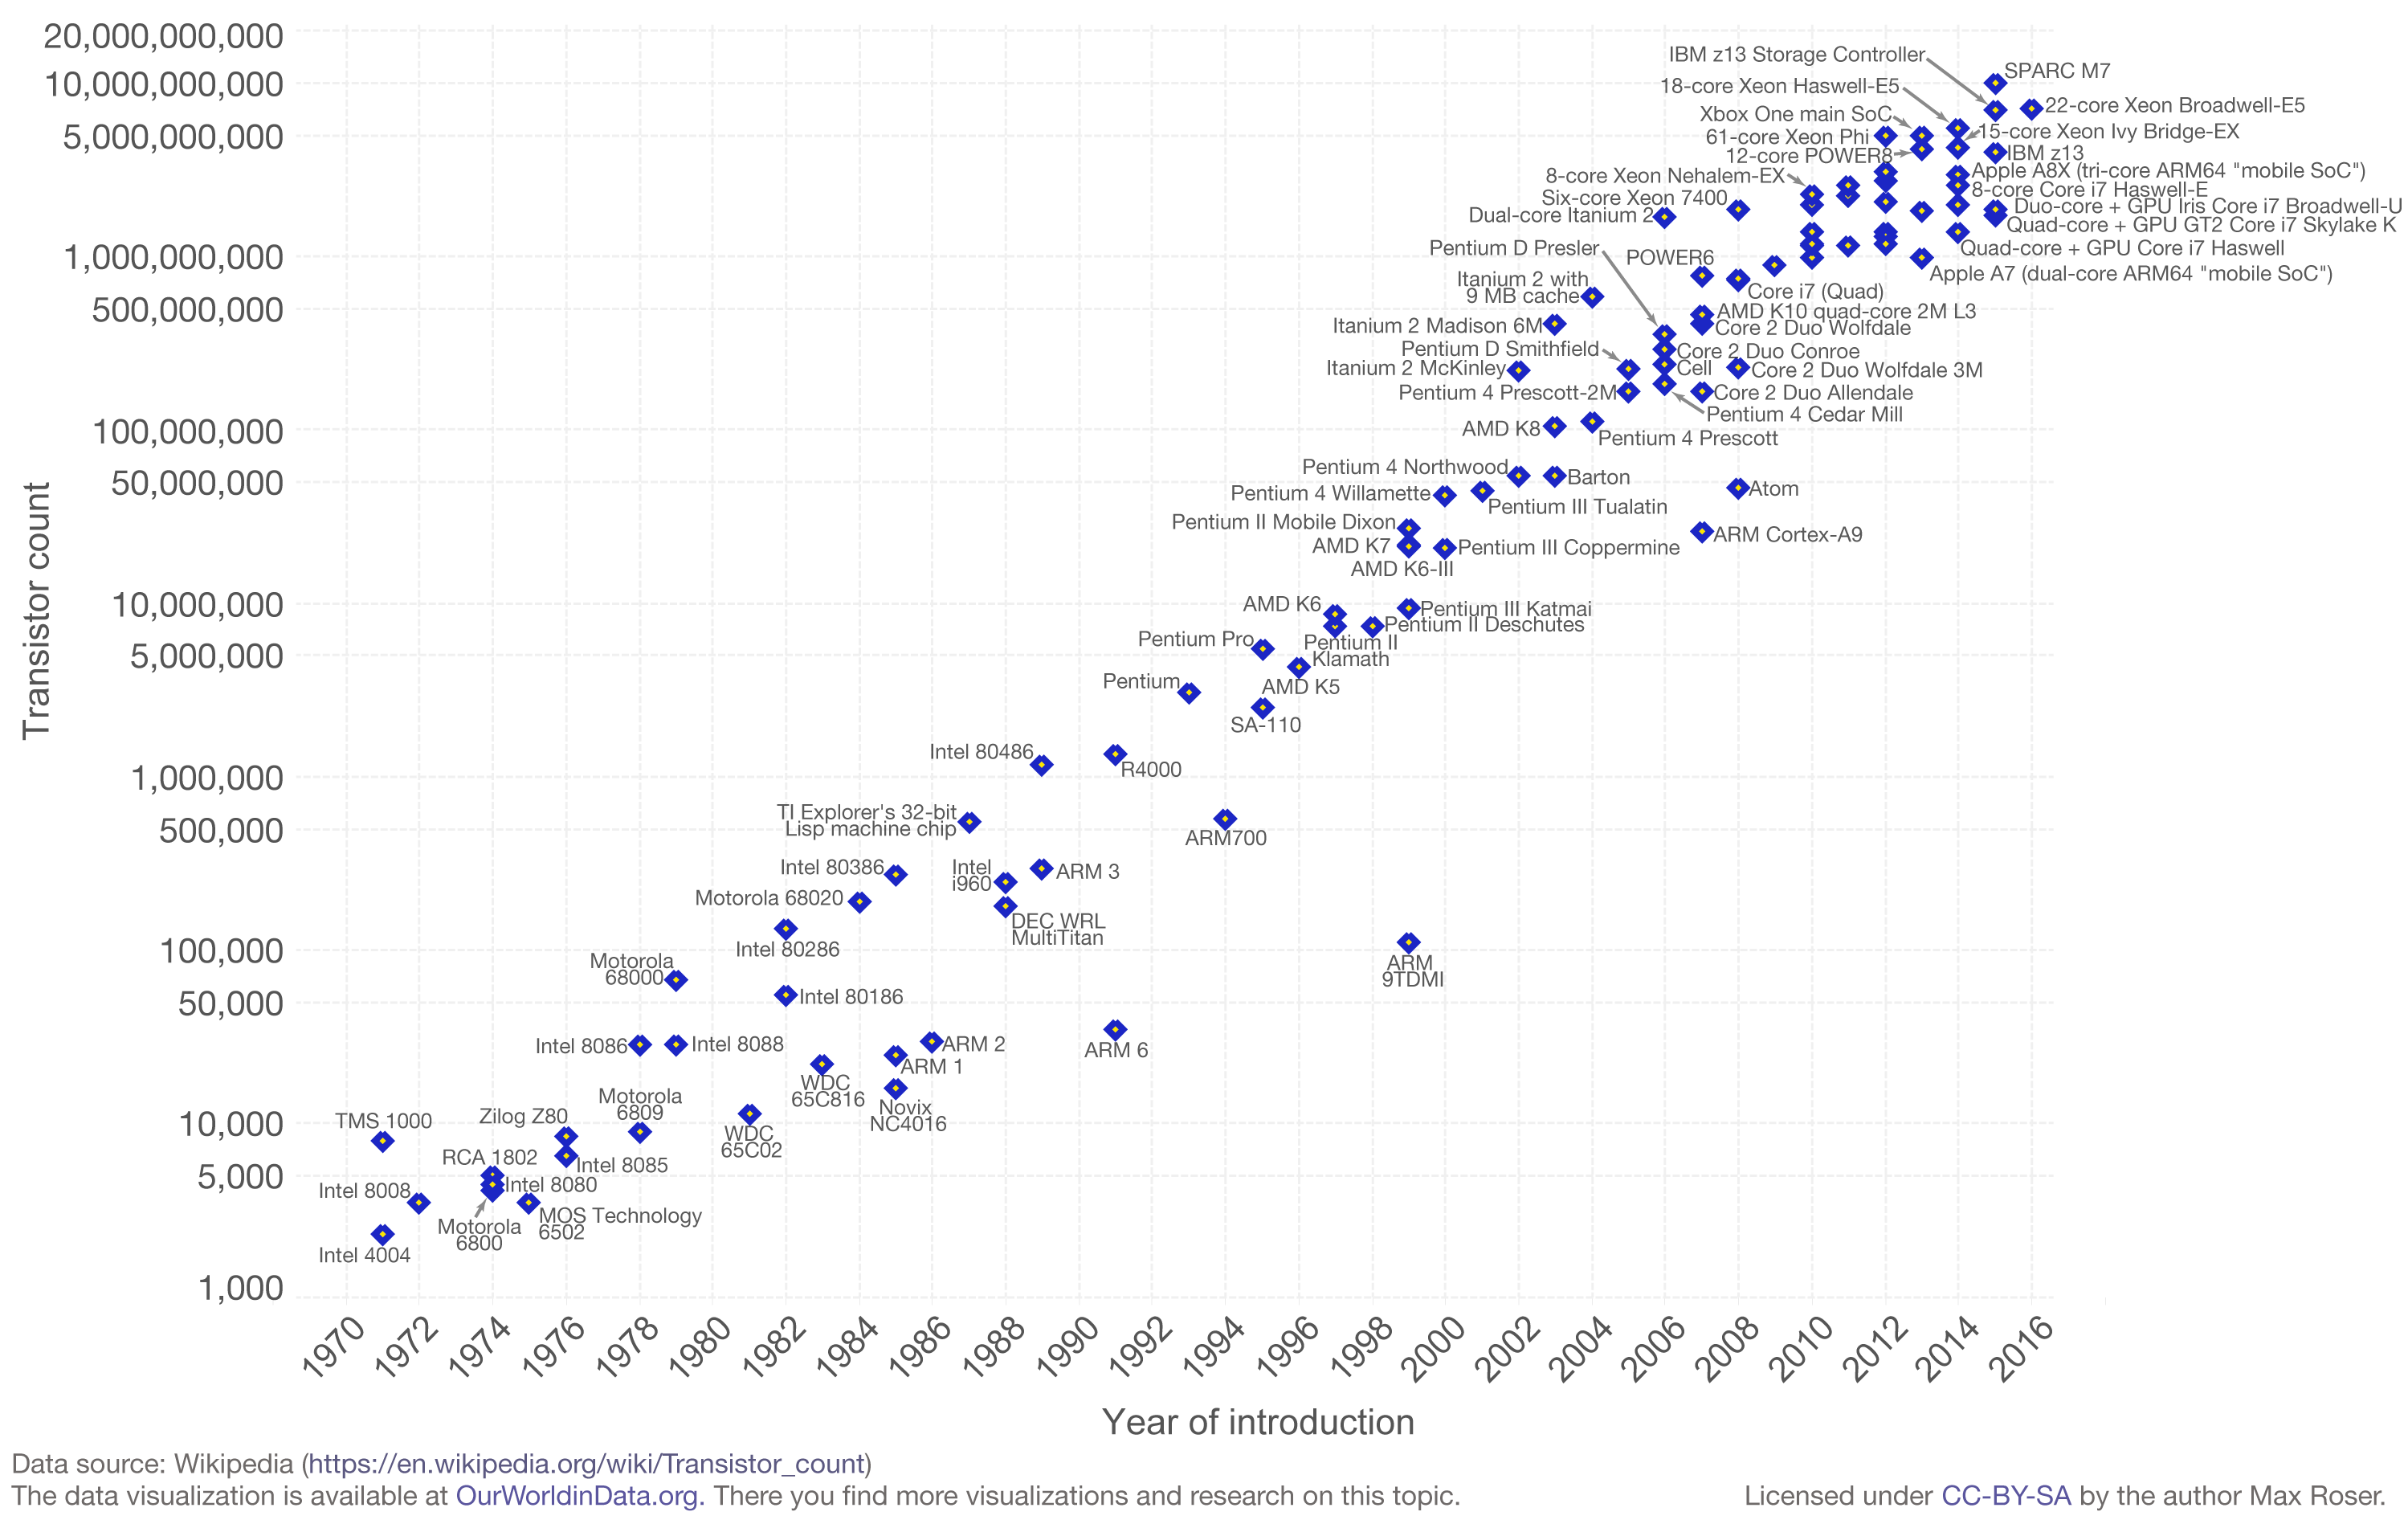
\includegraphics[width = \linewidth]{Moores_Law.png}
	\caption{Chart showing Moore's law, with a logarithmic increase in transistor 	count on each chip from 1970-2016.}
	\label{fig:Moore's_Law}
\end{figure}

In fact, this feature is already used in so-called quantum annealers such as those built by D-Wave \cite{D-Wave}. These machines use tunneling to find optimal solutions to a range of optimisation problems, where  This example of tunnelling is related to the so-called `wave-particle duality' which is the second key feature of quantum mechanics. The distinction between waves and particles, whose behaviour is well established in classical physics, becomes blurred. Every object in the universe, depending on their energy and confinement, will display both of these aspects to some degree. \\

The tantalising promise of quantum computing is hidden in this property. Particles such as electrons, which have comprised the backbone of electricity and classical information for the past century, have the ability to behave in a wave-like manner: they could contain not just the binary bit choices of 0 or 1,  but one of an infinite number of continuous values, called `qubits'. The ability to investigate the effect of a process on both 0 and 1 bits simultaneously means that quantum computers have the ability to scale exponentially (instead of polynomially) with the resources  that are put in. This scaling is crucial. Currently for computationally difficult tasks (problems in science, AI and more) supercomputers must be used, which take up massive amounts of space and are costly to build and run. The current state of the art is shown in  \autoref{fig:Summit}. If instead our computational scaling was exponential instead of polynomial we could perform the same task with many fewer qubits than bits - as the problem becomes more exaggerated \footnote{A classic example of the power of exponential scaling is given by the legend of a vizier who presented a gift to his King. The king asked what he wanted in return, and the vizier replied that he wanted rice. Precisely, he wanted one grain of rice on the first square of the chessboard, two grains of rice on the second, four grains on the third, and so on, doubling on each square. This bankrupts the king, who has to find $2^{63}$ grains of rice for the last square alone. This is $\sim 100$ times greater than the \emph{current} global annual food production. (At $\sim 10^{12}$kg \cite{Globalfoodproduction})}. Combined with entanglement to allow our qubits to influence each other in these states, we can harness a form of parallelism that results from the wave-like nature of controlled particles.  \\

While in general it is doubtful that a quantum computer will be universally  `faster' than a classical computer, and is much harder to engineer, there is significant potential to outperform conventional computers at certain tasks. While the amount of information processing in a conventional computer scales linearly with the number of bits, a quantum computer scales exponentially with the number of qubits for these tasks. Thus adding a single extra qubit could double the computing power. These are discussed, along with the quantum algorithms used to implement them, in \autoref{Algorithmsandapplications}. At the point when quantum computers are able to outperform classical supercomputers at a task, the so-called `quantum supremacy' \cite{Preskill2012} will have been achieved. \\

% are we mentioning that we can simulate around 50-qubit Q computer with classical computers?

% Further references on Q supremacy. First time defined \cite{Preskill2012}, recently proposed algorithm \cite{QKitchenSinks2018}, theoretical work on the amount of qubits needed for it \cite{Harrow2018}, the article suggesting supremacy with Boson sampling is far away \cite{BSsupremacy2017}.

These tasks range from aiding the fields of medicine, chemistry and materials with applications including creating more powerful simulations\footnote{This application - the simulation of large, complex many body systems - was in fact one of the very first motivators for the development of quantum computers, most famously by Richard Feynman \cite{Feynman1982simulating}.}\cite{Georgescu2014Sim}; providing potential speedups for AI and machine learning \cite{Biamonte2017QML}; assisting with modelling complex logistics problems; and improving financial models \cite{Schaden2002quantumfinance}.\\

However, achieving this potential does not come without significant engineering difficulties. Readout or detection of the information in the qubit destroys the information contained within, resulting in us reverting to the classical bit values with an some probabilities. These probabilities  are a fundamental (and irremovable) part of quantum theory, providing the link between \ldots Furthermore, the technology is still very young and undeveloped. Algorithms exist for many of the applications above, but there may be many more as yet undiscovered. Academic institutions, large corporations (including Google \cite{googleqai, bristlecone}, IBM, \cite{ibmqweb} and Intel \cite{intelqcomp}) and small start-ups, sucha as Rigetti, \cite{rigettihome}, alike have invested heavily in hardware. There are a wide range of platforms and architectures, including but not limited to superconducting qubits \cite{bristlecone}, ion traps \cite{steane1997ionTrap}, quantum dots \cite{loss1998quantumdots}, spin qubits in silicon \cite{intelSCspinqubits}, and silicon poisson bullets \cite{RudolphSiliconPhotonicsQC}. \\

\begin{figure}
    \centering
    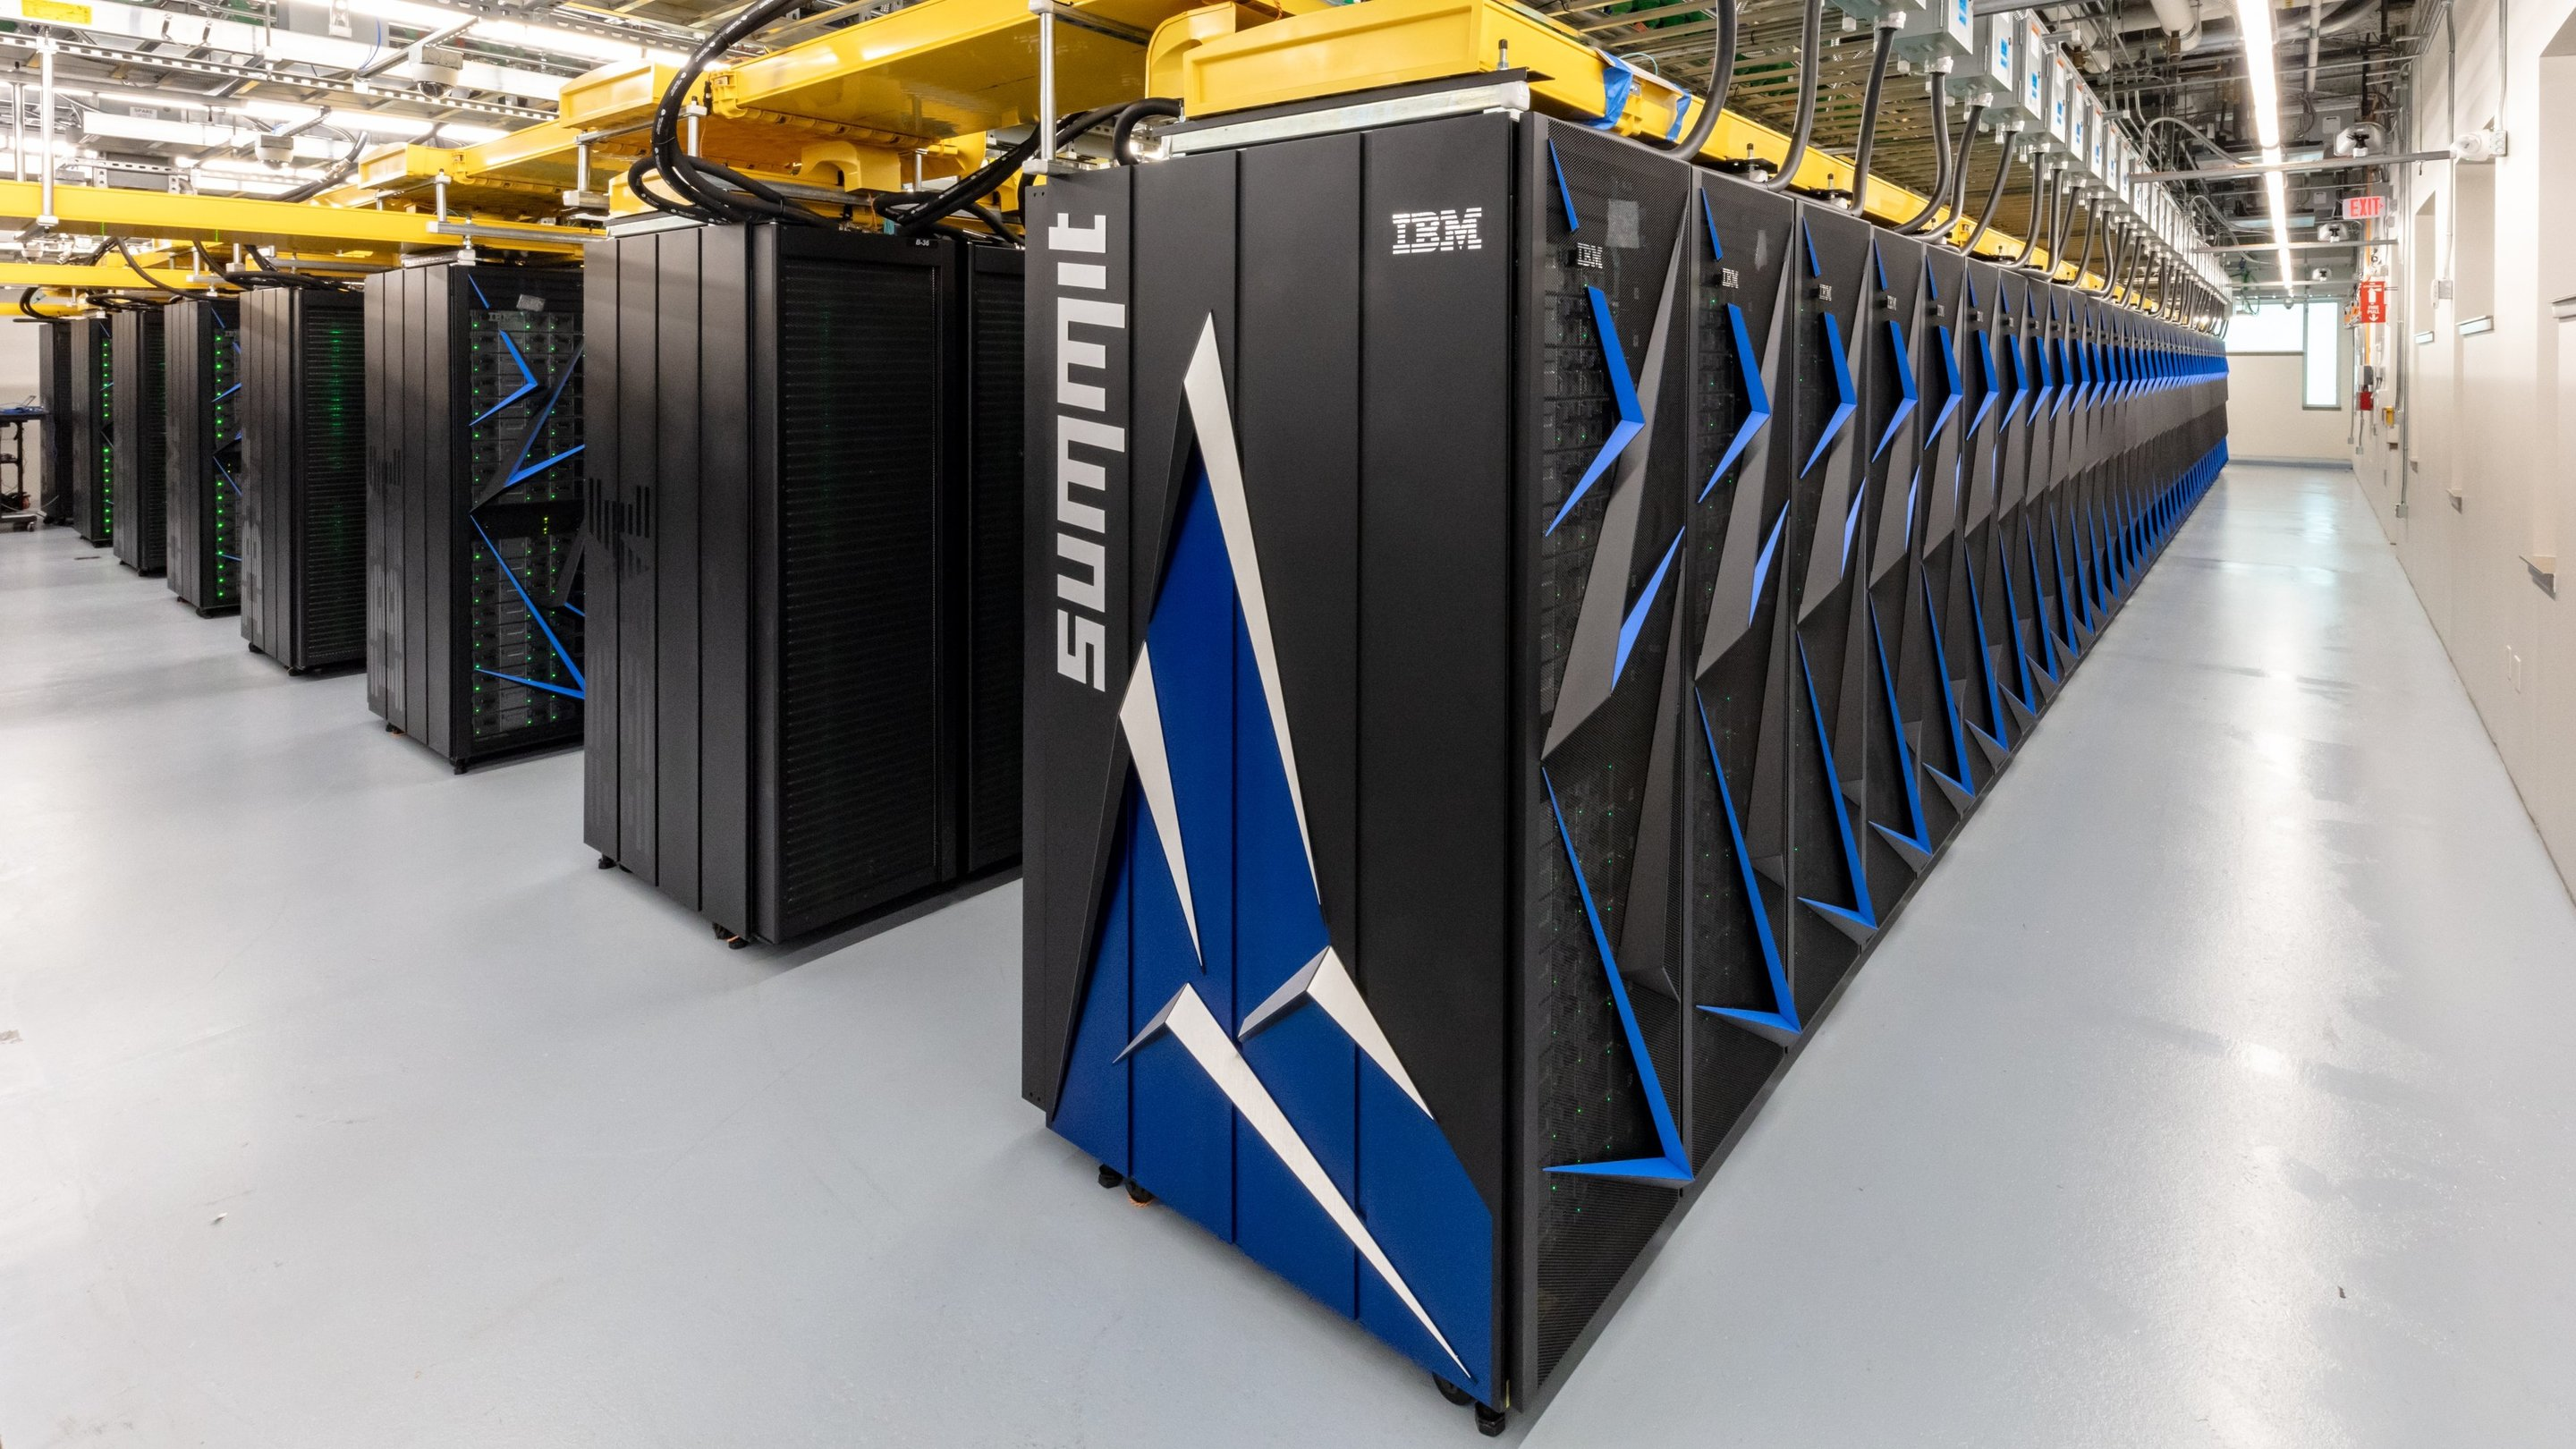
\includegraphics[width=\linewidth]{figures/SummitSC.jpg}
    \caption{The summit supercomputer, currently set to be the worlds fastest supercomputer, taking up the area of two tennis courts. \cite{SummitSC}}
    \label{fig:Summit}
\end{figure}

One crucial area that remains comparatively underdeveloped is software. It will be crucial to provide the missing link between theoretical algorithm and their implementation on a quantum computer. Ideally `quantum programming' should adopt many of the features as its classical counterpart: it should be usable by any person without understanding the details of the hardware being used, while allowing access to the fundamental workings of the computer. However, all programming languages will have to trade off these two features to some degree. Finally it is required to translate the input of the user into a set of instructions that the computer can follow efficiently. This step is called compilation and is crucial to the ability to use computers.

On the other hand, several attempts to  \cite{AlamosIBM2018, Xanadu2018, DK2018, DKBlog, RL2018, JW2018}. However, these documents have often focused on one or two languages. In this guide, we intend to keep a broad overview of the current state of the languages out there. In particular, in the manner of conventional programming guides, we provide many worked examples and problems to aid newcomers to the field. 

%%%%%%%%%%%%%%%
\begin{comment}

There are alraedy several quantum programming languages in place, in this guide we are going to address pyquil by, QISKit by IBM, project Q and Q\#

also citing benchmarking \cite{JW2018}. Our guide is similar to \cite{RL2018} as in we are going to be comparing specific algorithm with different languages, the differences are this and that also all code in jupyter notebooks.

More resources for each programming language

Forest more Resources. pyQUIL other guides and resources. There are already programming guides addressing the use of pyQuil \cite{DK2018} and his blog \cite{DKBlog}.

QISKit more resoruces  \cite{IBM2018}.  \cite{RL2018}. 

Project Q more resources  \cite{RL2018}. 

Q\# more resources (ADD REFERENCES FOR OTHER GUIDES HERE)

REFERENCES for further languages compile this which we briefly describe at the end. \cite{Xanadu2018} \cite{IonQ}

\end{comment}
%%%%%%%%%%%%%


Over the next few years and decades quantum computing is likely to become a reality, eventually becoming accessible to people from a range of disciplines via cloud services. It will be crucial when this becomes the case that people are able to understand how to use these machines in order to harness their applicability to the areas of mathematics, computer science, chemistry and finance. This guide is designed to be an introduction to the science of quantum computers and the current state of the field. Initially we explain in more depth how quantum computers work and their differences to classical computers in \autoref{TheBasics}. Since in the short-term, quantum computers are likely to be noisy, error-prone and limited in scale, we discuss how they can be used in this regime in \autoref{Shortqcomp}. \\

Once the engineering of quantum computers have been improved, then a host of more impressive applications can be demonstrated, which are considered in \autoref{Algorithmsandapplications}. We examine the programming languages that will be able to interface between the algorithms and the quantum computer in \autoref{Programmingquantumcomputer}, and hardware-specific implementations and architectures in \autoref{Implementations}. \\

A more complete description of quantum mechanics is given in \autoref{Advancedtopics} for any interested party. 
